\section{Results}

This section presents the key outcomes from the development and initial testing of the HealthHub platform. We focused on evaluating the core functionalities, user interface effectiveness, and the performance of the AI-driven food safety and nutritional analysis features, particularly those concerning FSSAI guidelines and personal health data.

\subsection{User Interface and Experience}
HealthHub provides a clean and intuitive user interface, designed to make complex health and food safety information accessible. Figure \ref{fig:hm-hero} showcases the platform's landing page, introducing users to HealthHub's capabilities.

\begin{figure}[!t]
\centering
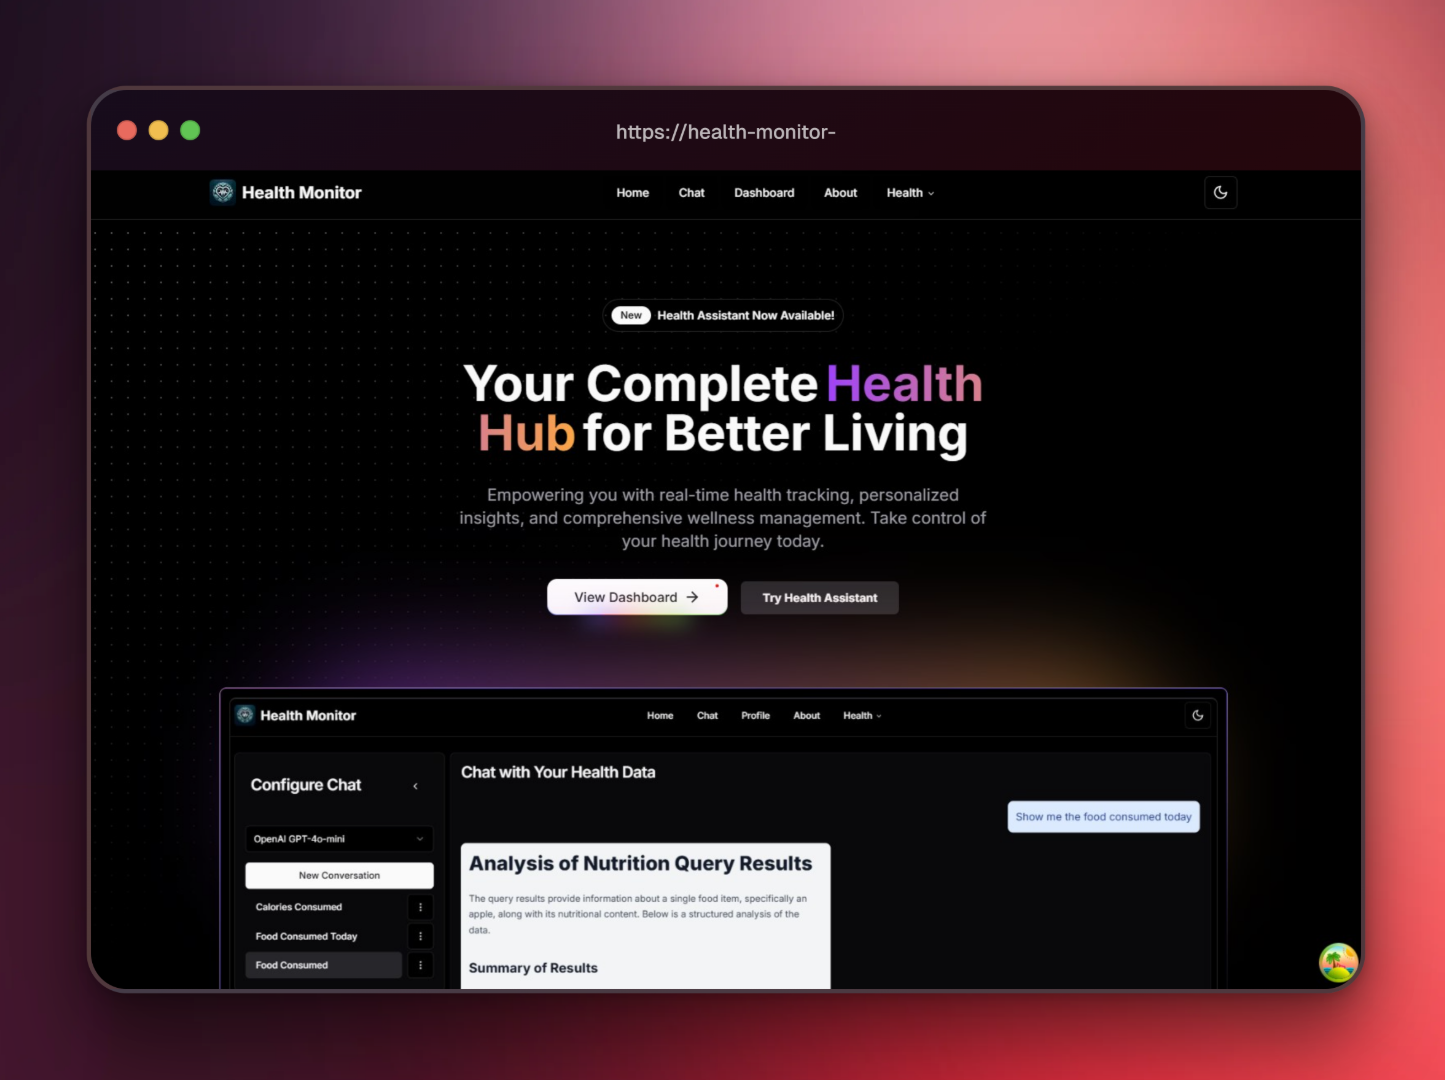
\includegraphics[width=0.9\columnwidth]{figures/hm-hero.png} % User to confirm/update path
\caption{The HealthHub landing page, highlighting its core features and value proposition to the user.}
\label{fig:hm-hero}
\end{figure}

Upon logging in, users are presented with the main dashboard (Figure \ref{fig:hm-dashboard}), which offers an overview of their logged data and quick access to various features, including food logging and initiating queries.

\begin{figure}[!t]
\centering
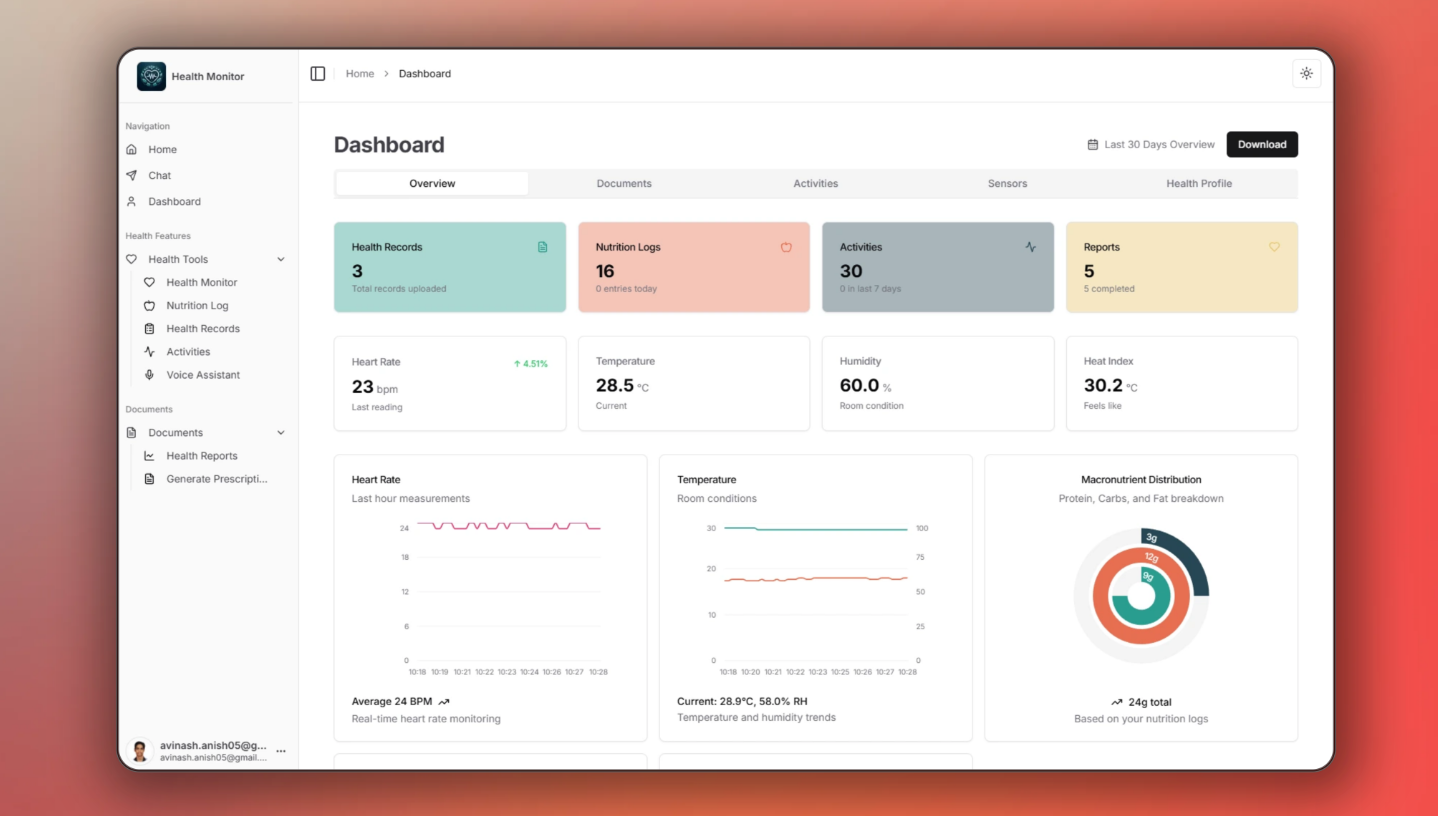
\includegraphics[width=0.9\columnwidth]{figures/hm-dashboard.png} % User to confirm/update path
\caption{The HealthHub main dashboard, providing a central point for users to view their health summary and access features.}
\label{fig:hm-dashboard}
\end{figure}

HealthHub supports multiple modalities for interacting with its AI assistant. Figure \ref{fig:hm-chat} illustrates the text-based chat interface. Furthermore, an integrated AI Voice and Video Assistant, shown in Figure \ref{fig:hm-video-assistant}, allows users to engage in spoken conversations and receive visual feedback from an AI avatar, enhancing the interactive experience.

\begin{figure}[!t]
\centering
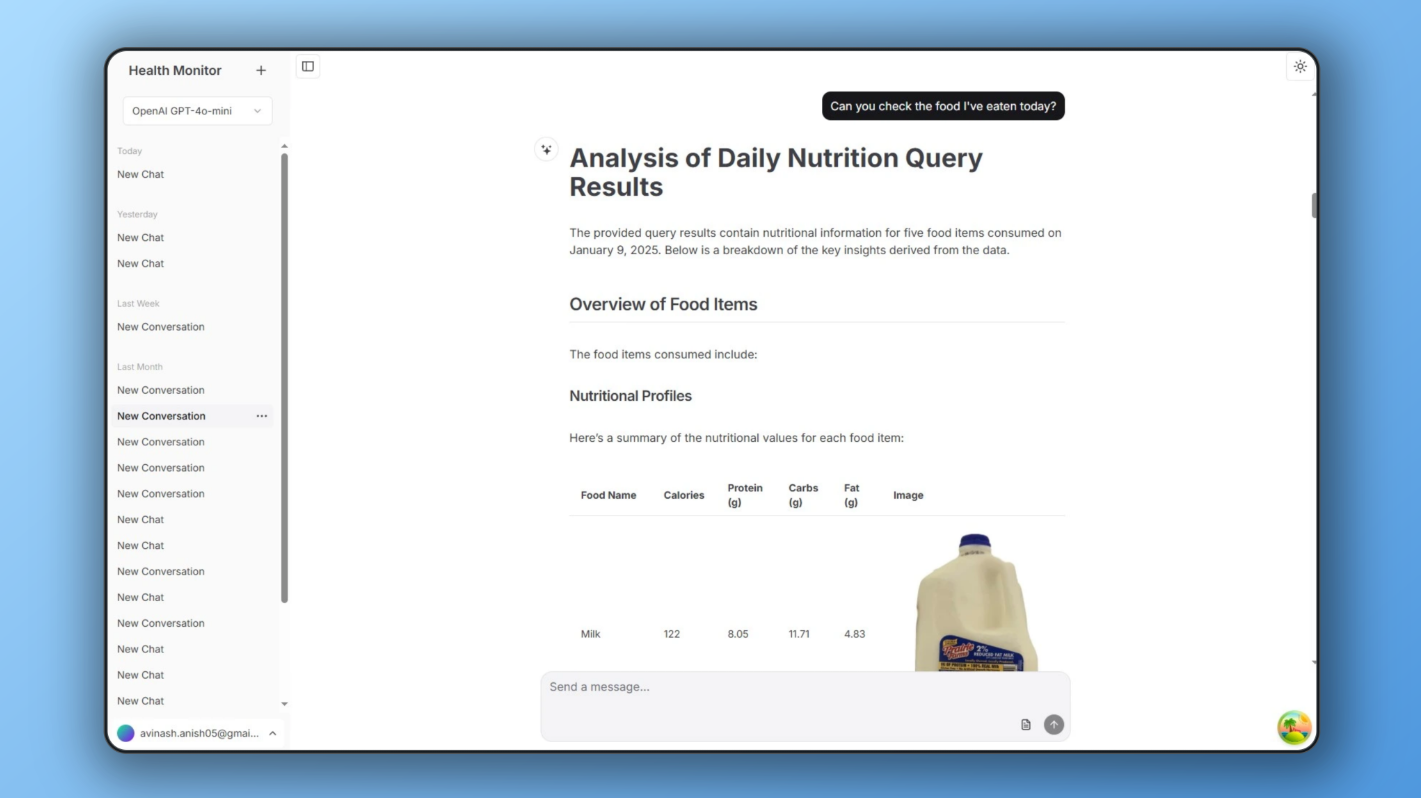
\includegraphics[width=0.9\columnwidth]{figures/hm-chat.png} % User to confirm/update path
\caption{HealthHub's text chat interface for querying the AI assistant about food safety, FSSAI guidelines, and nutrition.}
\label{fig:hm-chat}
\end{figure}

\begin{figure}[!t]
\centering
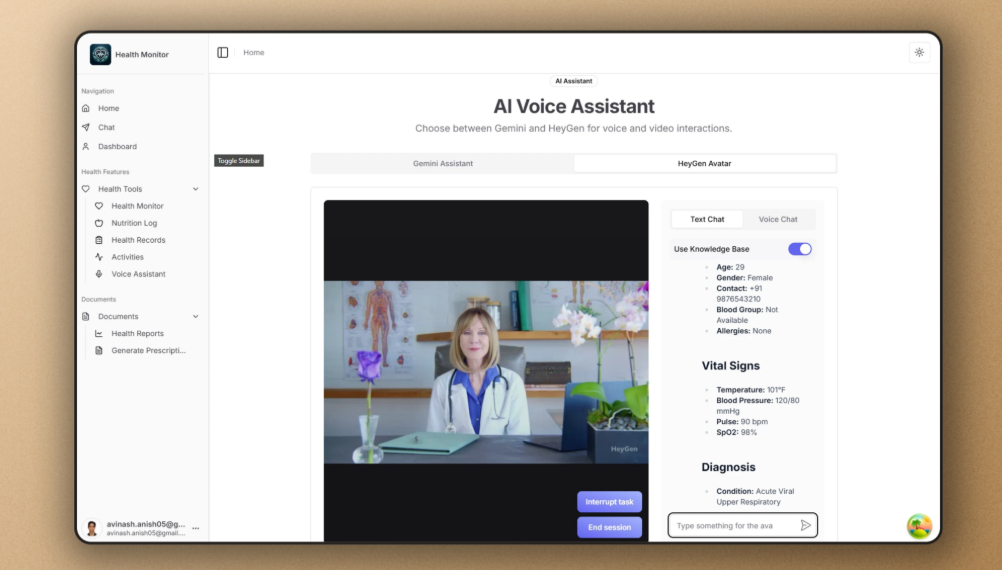
\includegraphics[width=0.8\columnwidth]{figures/hm-video.png} % Changed from 0.7, user to confirm filename (hm-video.png or specific AI assistant image)
\caption{The HealthHub AI Voice and Video Assistant interface, enabling spoken interaction and visual feedback.}
\label{fig:hm-video-assistant}
\end{figure}

\subsection{AI-Powered Food Safety and Nutritional Analysis}
Our AI core, combining a RAG pipeline and an SQL agent, demonstrated its ability to provide relevant and personalized information. Table \ref{tab:rag-examples} presents illustrative examples of the RAG pipeline addressing FSSAI and food safety queries.

\begin{table}[!ht]
\centering
\caption{Illustrative FSSAI & Food Safety Queries (RAG Pipeline)}
\label{tab:rag-examples}
\begin{tabular}{|p{0.4\columnwidth}|p{0.5\columnwidth}|}
\hline
\textbf{User Query/Scenario} & \textbf{HealthHub Response (Illustrative)} \\
\hline
User types: "Are there FSSAI rules for using artificial sweeteners in baked goods?" & Yes, FSSAI's Food Safety and Standards (Food Products Standards and Food Additives) Regulations, 2011, specify approved artificial sweeteners like Aspartame and Sucralose for use in baked goods, within prescribed maximum limits. For example, Aspartame is permitted up to 1000 mg/kg in certain bakery products. It's important to check product labels for declarations. \\
\hline
User asks: "What does FSSAI say about pesticide residues in fruits?" & FSSAI has established Maximum Residue Limits (MRLs) for various pesticides in different food commodities, including fruits, under the Food Safety and Standards (Contaminants, Toxins and Residues) Regulations, 2011. These limits are regularly reviewed. For specific fruits, it's best to refer to the latest FSSAI notifications on MRLs. \\
\hline
\end{tabular}
\end{table}

Table \ref{tab:sql-agent-examples} showcases the SQL agent processing natural language queries against logged dietary data.

\begin{table}[!ht]
\centering
\caption{Illustrative Personalized Nutritional Insights (SQL Agent)}
\label{tab:sql-agent-examples}
\begin{tabular}{|p{0.4\columnwidth}|p{0.5\columnwidth}|}
\hline
\textbf{User Query/Scenario} & \textbf{HealthHub Response (Illustrative)} \\
\hline
User asks via voice: "HealthHub, what was my average daily sugar intake this past week?" & Based on your logged food items from the past week, your average daily sugar intake was approximately 65 grams. The World Health Organization recommends adults consume no more than 25-50 grams of free sugars per day for optimal health. \\
\hline
User types: "Compare my protein intake yesterday with the day before." & Yesterday, your protein intake was 70g. The day before, it was 55g. You consumed 15g more protein yesterday. \\
\hline
\end{tabular}
\end{table}

\subsection{Sensor Data Integration and Alert Potential}
The sensor subsystem successfully logged physiological data (e.g., heart rate, SpO2 from MAX30102) to the user's profile. This data enables correlational analysis, as illustrated in Table \ref{tab:sensor-alert-example}.

\begin{table}[!ht]
\centering
\caption{Illustrative Sensor Data Correlation and Advisory}
\label{tab:sensor-alert-example}
\begin{tabular}{|p{0.4\columnwidth}|p{0.5\columnwidth}|}
\hline
\textbf{System Trigger/Scenario} & \textbf{HealthHub Advisory (Illustrative)} \\
\hline
User logs consumption of a highly caffeinated energy drink. System correlates this with sensor data showing a heart rate increase from baseline 70 bpm to 105 bpm, sustained for 45 minutes. & Noticed a significant heart rate increase after your logged energy drink. Frequent high caffeine intake can impact cardiovascular health. Consider moderation. \\
\hline
\end{tabular}
\end{table}

\subsection{System Performance and Responsiveness}
Initial evaluations indicate that HealthHub is responsive. Queries to the RAG pipeline for FSSAI information were typically answered within 3-5 seconds. The SQL agent also demonstrated efficient query execution for nutritional summaries, usually taking less than 2 seconds. While formal benchmarking is ongoing, the current performance supports an engaging user experience. 